% =========================
% CHƯƠNG 4
% =========================
\chapter{Kiến trúc hệ thống}

\section{Thiết kế tổng thể}

Hệ thống điều khiển đèn giao thông thông minh được xây dựng theo mô hình phân tầng, kết hợp giữa điều khiển dựa trên luật (rule-based) và học tăng cường bằng máy (reinforcement learning). Kiến trúc này đảm bảo hệ thống vừa ổn định, an toàn, vừa có khả năng thích ứng và tối ưu theo trạng thái giao thông thực tế.

\subsection{Sơ đồ thành phần hệ thống}

\begin{figure}[H]
    \centering
    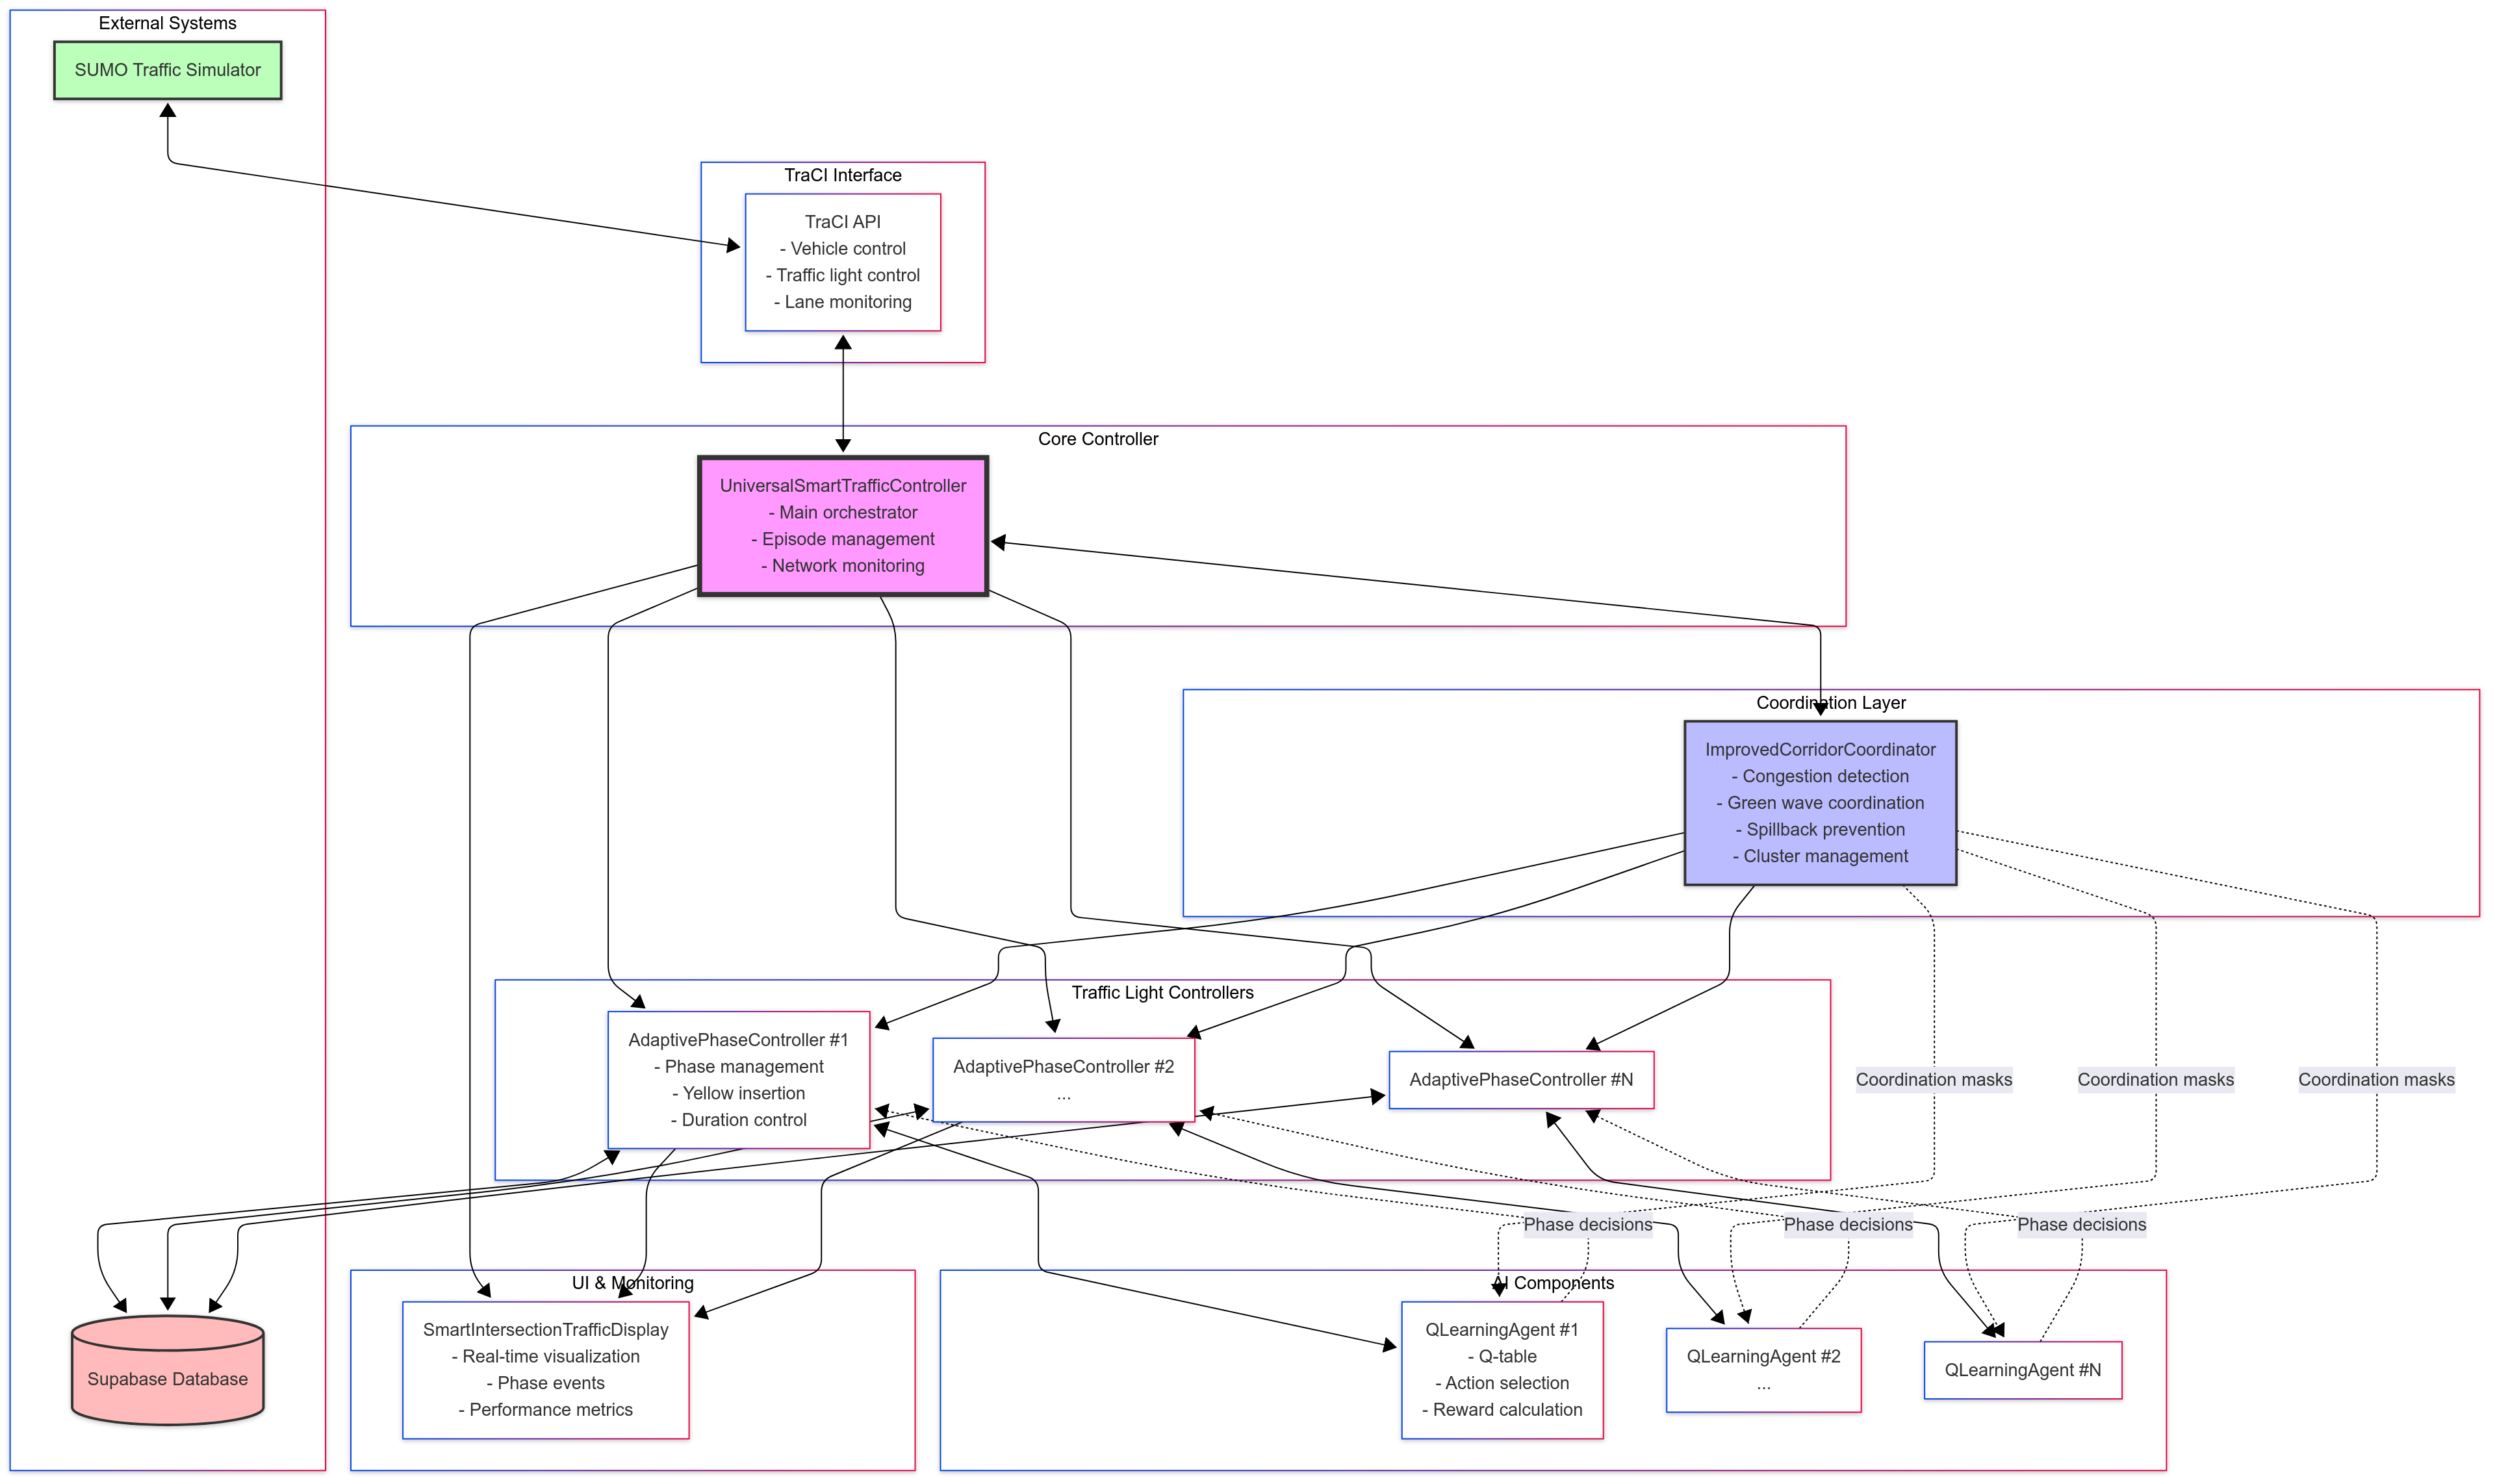
\includegraphics[width=1\linewidth]{Untitled diagram _ Mermaid Chart-2025-08-21-023904.png}
    \caption{Kiến trúc tổng thể hệ thống điều khiển đèn giao thông}
\end{figure}

Hệ thống gồm 4 tầng chính:
\begin{itemize}
    \item \textbf{Tầng mô phỏng}: Sử dụng SUMO làm môi trường giao thông vi mô, cung cấp dữ liệu thời gian thực về phương tiện, làn đường, đèn tín hiệu.
    \item \textbf{Tầng giao tiếp}: TraCI làm cầu nối hai chiều giữa SUMO và hệ điều khiển Python, cho phép truy vấn trạng thái và gửi lệnh điều khiển.
    \item \textbf{Tầng điều khiển}: UniversalSmartTrafficController quản lý một nút giao, điều phối các AdaptivePhaseController (APC) và RL agent để ra quyết định động, xử lý ưu tiên, tắc nghẽn, rẽ trái bảo vệ.
    \item \textbf{Tầng lưu trữ}: Supabase lưu trữ trạng thái, log sự kiện, lịch sử pha và Q-table; pickle file lưu Q-table cục bộ giúp agent khôi phục trạng thái học.
\end{itemize}

\section{Luồng dữ liệu và tích hợp}

Quy trình dữ liệu của hệ thống theo chu trình khép kín:
\begin{enumerate}
    \item TraCI đọc trạng thái giao thông từ SUMO (số lượng xe, hàng chờ, tốc độ...).
    \item UniversalSmartTrafficController tổng hợp, phân tích dữ liệu, đánh giá trạng thái nút giao.
    \item AdaptivePhaseController và RL agent quyết định chuyển pha, điều chỉnh thời lượng theo trạng thái và lịch sử học.
    \item Lệnh điều khiển gửi ngược về SUMO qua TraCI.
    \item Kết quả, phần thưởng, log sự kiện được ghi lên Supabase, Q-table được cập nhật để cải thiện hiệu năng lâu dài.
\end{enumerate}

Các điểm tích hợp chính:
\begin{itemize}
    \item \textbf{TraCI API}: Giao tiếp và thao tác trạng thái với SUMO, tối ưu hóa qua subscription.
    \item \textbf{Supabase REST API}: Đồng bộ trạng thái, log, Q-table lên cloud với batch write, retry logic.
    % \item \textbf{Corridor Coordinator}: Điều phối đa nút giao, phát hiện cluster congestion, tạo green wave.
    % Đã loại bỏ, vì hệ thống hiện tại chỉ điều khiển một nút giao.
\end{itemize}

\section{Các thành phần cốt lõi}

\subsection{UniversalSmartTrafficController}

Điều khiển trung tâm, quản lý APC cho một nút giao, thu thập và phân tích dữ liệu, nhận diện các tình huống đặc biệt (ưu tiên, tắc nghẽn, starvation).

\subsection{AdaptivePhaseController (APC)}

Điều khiển nút giao, thực hiện điều chỉnh động thời lượng pha, chèn pha vàng, bảo vệ rẽ trái, xử lý hàng đợi ưu tiên, phối hợp với RL agent và controller.

\subsection{EnhancedQLearningAgent}

Tác tử học tăng cường Q-learning, nhận vector trạng thái đa chiều, cập nhật Q-table, tối ưu hóa lựa chọn pha và thời lượng dựa trên reward đa mục tiêu.

\subsection{Giao tiếp SUMO–TraCI}

Các hàm bọc giúp kiểm soát pha an toàn, cache logic đèn tín hiệu (TTL 0.5s), quản lý subscription giảm overhead truyền tin, đảm bảo quá trình điều khiển ổn định.

\section{Công nghệ sử dụng}

\subsection{Python và thư viện}

Hệ thống phát triển trên Python 3.8+:
\begin{itemize}
    \item \textbf{Async/Await, Threading}: Xử lý bất đồng bộ, tăng hiệu suất
    \item \textbf{Type Hints, Dataclasses}: Quản lý dữ liệu rõ ràng, dễ bảo trì
    \item \textbf{NumPy, Pandas, Matplotlib}: Phân tích, xử lý và trực quan hóa dữ liệu
    \item \textbf{Supabase-py}: Kết nối cloud database
    \item \textbf{Pickle}: Lưu/đọc Q-table cục bộ
\end{itemize}

\subsection{Mô phỏng giao thông SUMO}

SUMO 1.22.0 với NETEDIT cho phép thiết kế mạng lưới, cấu hình traffic demand, xuất dữ liệu chi tiết phục vụ kiểm thử và đào tạo.

\subsection{Tích hợp API TraCI}

Các module chính:
\begin{itemize}
    \item \texttt{traci.trafficlight}: Điều khiển pha, logic đèn
    \item \texttt{traci.lane}: Đọc thông tin làn, hàng chờ
    \item \texttt{traci.vehicle}: Theo dõi phương tiện
    \item \texttt{traci.simulation}: Quản lý mô phỏng chung
\end{itemize}

\subsection{Cấu hình Supabase}

Supabase sử dụng PostgreSQL cloud với REST API và real-time. Hệ thống tối ưu hóa lưu trữ và truy vấn dữ liệu bằng cấu trúc bảng sau:

\subsubsection{Bảng apc\_states}

Lưu trữ trạng thái tổng thể APC, bao gồm cấu hình pha, hàng đợi sự kiện, trạng thái RL agent.

\begin{lstlisting}[style=sql,caption={Định nghĩa bảng apc\_states}]
CREATE TABLE apc_states (
    id BIGSERIAL PRIMARY KEY,
    tls_id TEXT NOT NULL,
    state_type TEXT NOT NULL,
    data JSONB NOT NULL,
    created_at TIMESTAMPTZ DEFAULT NOW(),
    updated_at TIMESTAMPTZ DEFAULT NOW()
);

CREATE INDEX idx_apc_states_tls_type ON apc_states(tls_id, state_type);
CREATE INDEX idx_apc_states_data ON apc_states USING gin(data);
\end{lstlisting}

Trường \texttt{state\_type} gồm:
\begin{itemize}
    \item \texttt{full}: Snapshot trạng thái toàn bộ APC
    \item \texttt{phase}: Thông tin chi tiết pha đèn
    \item \texttt{event}: Sự kiện điều khiển đơn lẻ
\end{itemize}
Sử dụng JSONB giúp mở rộng dữ liệu linh hoạt, truy vấn nhanh nhờ GIN index, dễ dàng tích hợp với Python.

\subsubsection{Bảng phase\_records}

Lưu lịch sử các lần điều chỉnh pha đèn, phục vụ phân tích hiệu năng và đào tạo RL agent.

\begin{table}[H]
\centering
\begin{tabular}{llp{7cm}}
\toprule
\textbf{Cột} & \textbf{Kiểu} & \textbf{Vai trò} \\
\midrule
tls\_id         & TEXT    & Định danh nút giao \\
phase\_idx      & INT     & Pha được điều chỉnh (0--11) \\
duration        & REAL    & Thời lượng thực tế \\
base\_duration  & REAL    & Thời lượng cơ sở \\
delta\_t        & REAL    & Mức điều chỉnh \\
extended\_time  & REAL    & Thời gian mở rộng \\
reward          & REAL    & Reward từ RL agent \\
sim\_time       & REAL    & Thời điểm mô phỏng \\
\bottomrule
\end{tabular}
\caption{Các trường cốt lõi của bảng phase\_records}
\end{table}

\subsubsection{Bảng simulation\_events}

Lưu mọi sự kiện đặc biệt: chuyển pha khẩn cấp, protected left, congestion, chuyển vàng, v.v.

\begin{itemize}
    \item \texttt{id}: Khóa chính
    \item \texttt{tls\_id}: ID đèn giao thông
    \item \texttt{event\_type}: Loại sự kiện
    \item \texttt{event\_date}: JSONB chi tiết sự kiện
    \item \texttt{sim\_time}: Thời điểm mô phỏng
    \item \texttt{created\_at}: Thời điểm tạo bản ghi
\end{itemize}

Ví dụ JSON:
\begin{lstlisting}[style=json]
{
    "action": "phase_duration_update",
    "phase": 209
}
\end{lstlisting}

\subsubsection{Tối ưu hiệu suất database}

\begin{itemize}
    \item \textbf{Indexing}: Composite index cho truy vấn nhanh
    \item \textbf{JSONB + GIN}: Truy vấn linh hoạt, hiệu suất cao
    \item \textbf{Row Level Security}: Bảo mật theo từng dòng dữ liệu
    \item \textbf{Batch operations}: Ghi dữ liệu theo lô giảm số lần round-trip
\end{itemize}

\begin{lstlisting}[style=sql]
ALTER TABLE apc_states ENABLE ROW LEVEL SECURITY;
CREATE POLICY "Enable all operations for authenticated users"
    ON apc_states FOR ALL USING (auth.role() = 'authenticated');
\end{lstlisting}

\subsubsection{Chiến lược đồng bộ dữ liệu}

\begin{itemize}
    \item Dữ liệu tạm thời gom vào \_pending\_db\_ops (tối đa 1000 bản ghi)
    \item AsyncSupabaseWriter ghi dữ liệu định kỳ lên Supabase (60s/batch)
    \item Retry logic thông minh, tối đa 6 lần, dùng exponential backoff
    \item Nếu Supabase offline, chuyển sang lưu local tạm thời
\end{itemize}

Thiết kế này giúp hệ thống an toàn, hiệu suất cao, sẵn sàng mở rộng cho thực nghiệm hoặc triển khai thực tế.
